\documentclass{article}

\usepackage{fontspec}
\setmainfont[ExternalLocation=./fonts/]{USDeclaration.ttf}
\setmonofont{Ubuntu}
\newfontfamily\Greek[Path=./fonts/]{porson.ttf}

\setlength\parindent{0pt}
\usepackage[left=0.5cm, right=0.5cm]{geometry}
\usepackage{setspace}

\usepackage{graphicx}
\renewcommand{\labelitemi}{
\includegraphics[width=0.02\textwidth]{icon.png}}
\usepackage{wallpaper}

\usepackage{hyperref}
\hypersetup{
    colorlinks=true,
    linkcolor=blue,
    filecolor=magenta,
    urlcolor=blue
}

\usepackage{tcolorbox}
\usepackage{tabularx}
\usepackage{array}
\usepackage{colortbl}
\tcbuselibrary{skins}

\definecolor{loeb-green}{HTML}{11B872}
\newcolumntype{Y}{>{\centering\arraybackslash}X}
\tcbset{inflection/.style={
    enhanced,
    colback=yellow!10!white,
    colframe=loeb-green!50!black,
    colbacktitle=loeb-green!40!white,
    coltitle=black,
    center title
}}

\tcbset{reference/.style={
    enhanced,
    halign=flush right,
    colback=loeb-green!40!white,
    colframe=loeb-green!50!black,
}}

\newfontfamily\German[Path=./fonts/]{BreitkopfFraktur.ttf}[Scale=1.5]

\renewcommand{\labelitemi}{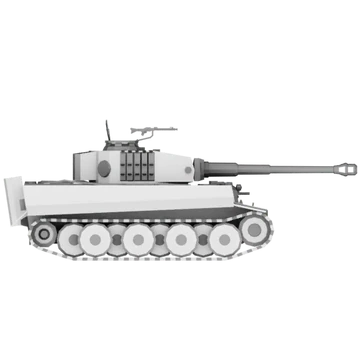
\includegraphics[width=0.05\textwidth]{german-item-icon}}

\definecolor{german-flag-red}{HTML}{DD0000}
\definecolor{german-flag-yellow}{HTML}{FFCC00}
\definecolor{german-flag-black}{HTML}{000000}
\newcolumntype{Y}{>{\centering\arraybackslash}X}
\tcbset{inflection/.style={
    enhanced,
    colback=german-flag-yellow!10!white,
    colframe=german-flag-black,
    colbacktitle=german-flag-red!50!white,
    coltitle=black,
    center title
}}

\tcbset{reference/.style={
    enhanced,
    halign=flush right,
    colback=german-flag-red!50!white,
    colframe=german-flag-black,
}}


\begin{document}
    \begin{figure}[H]
        \centering
        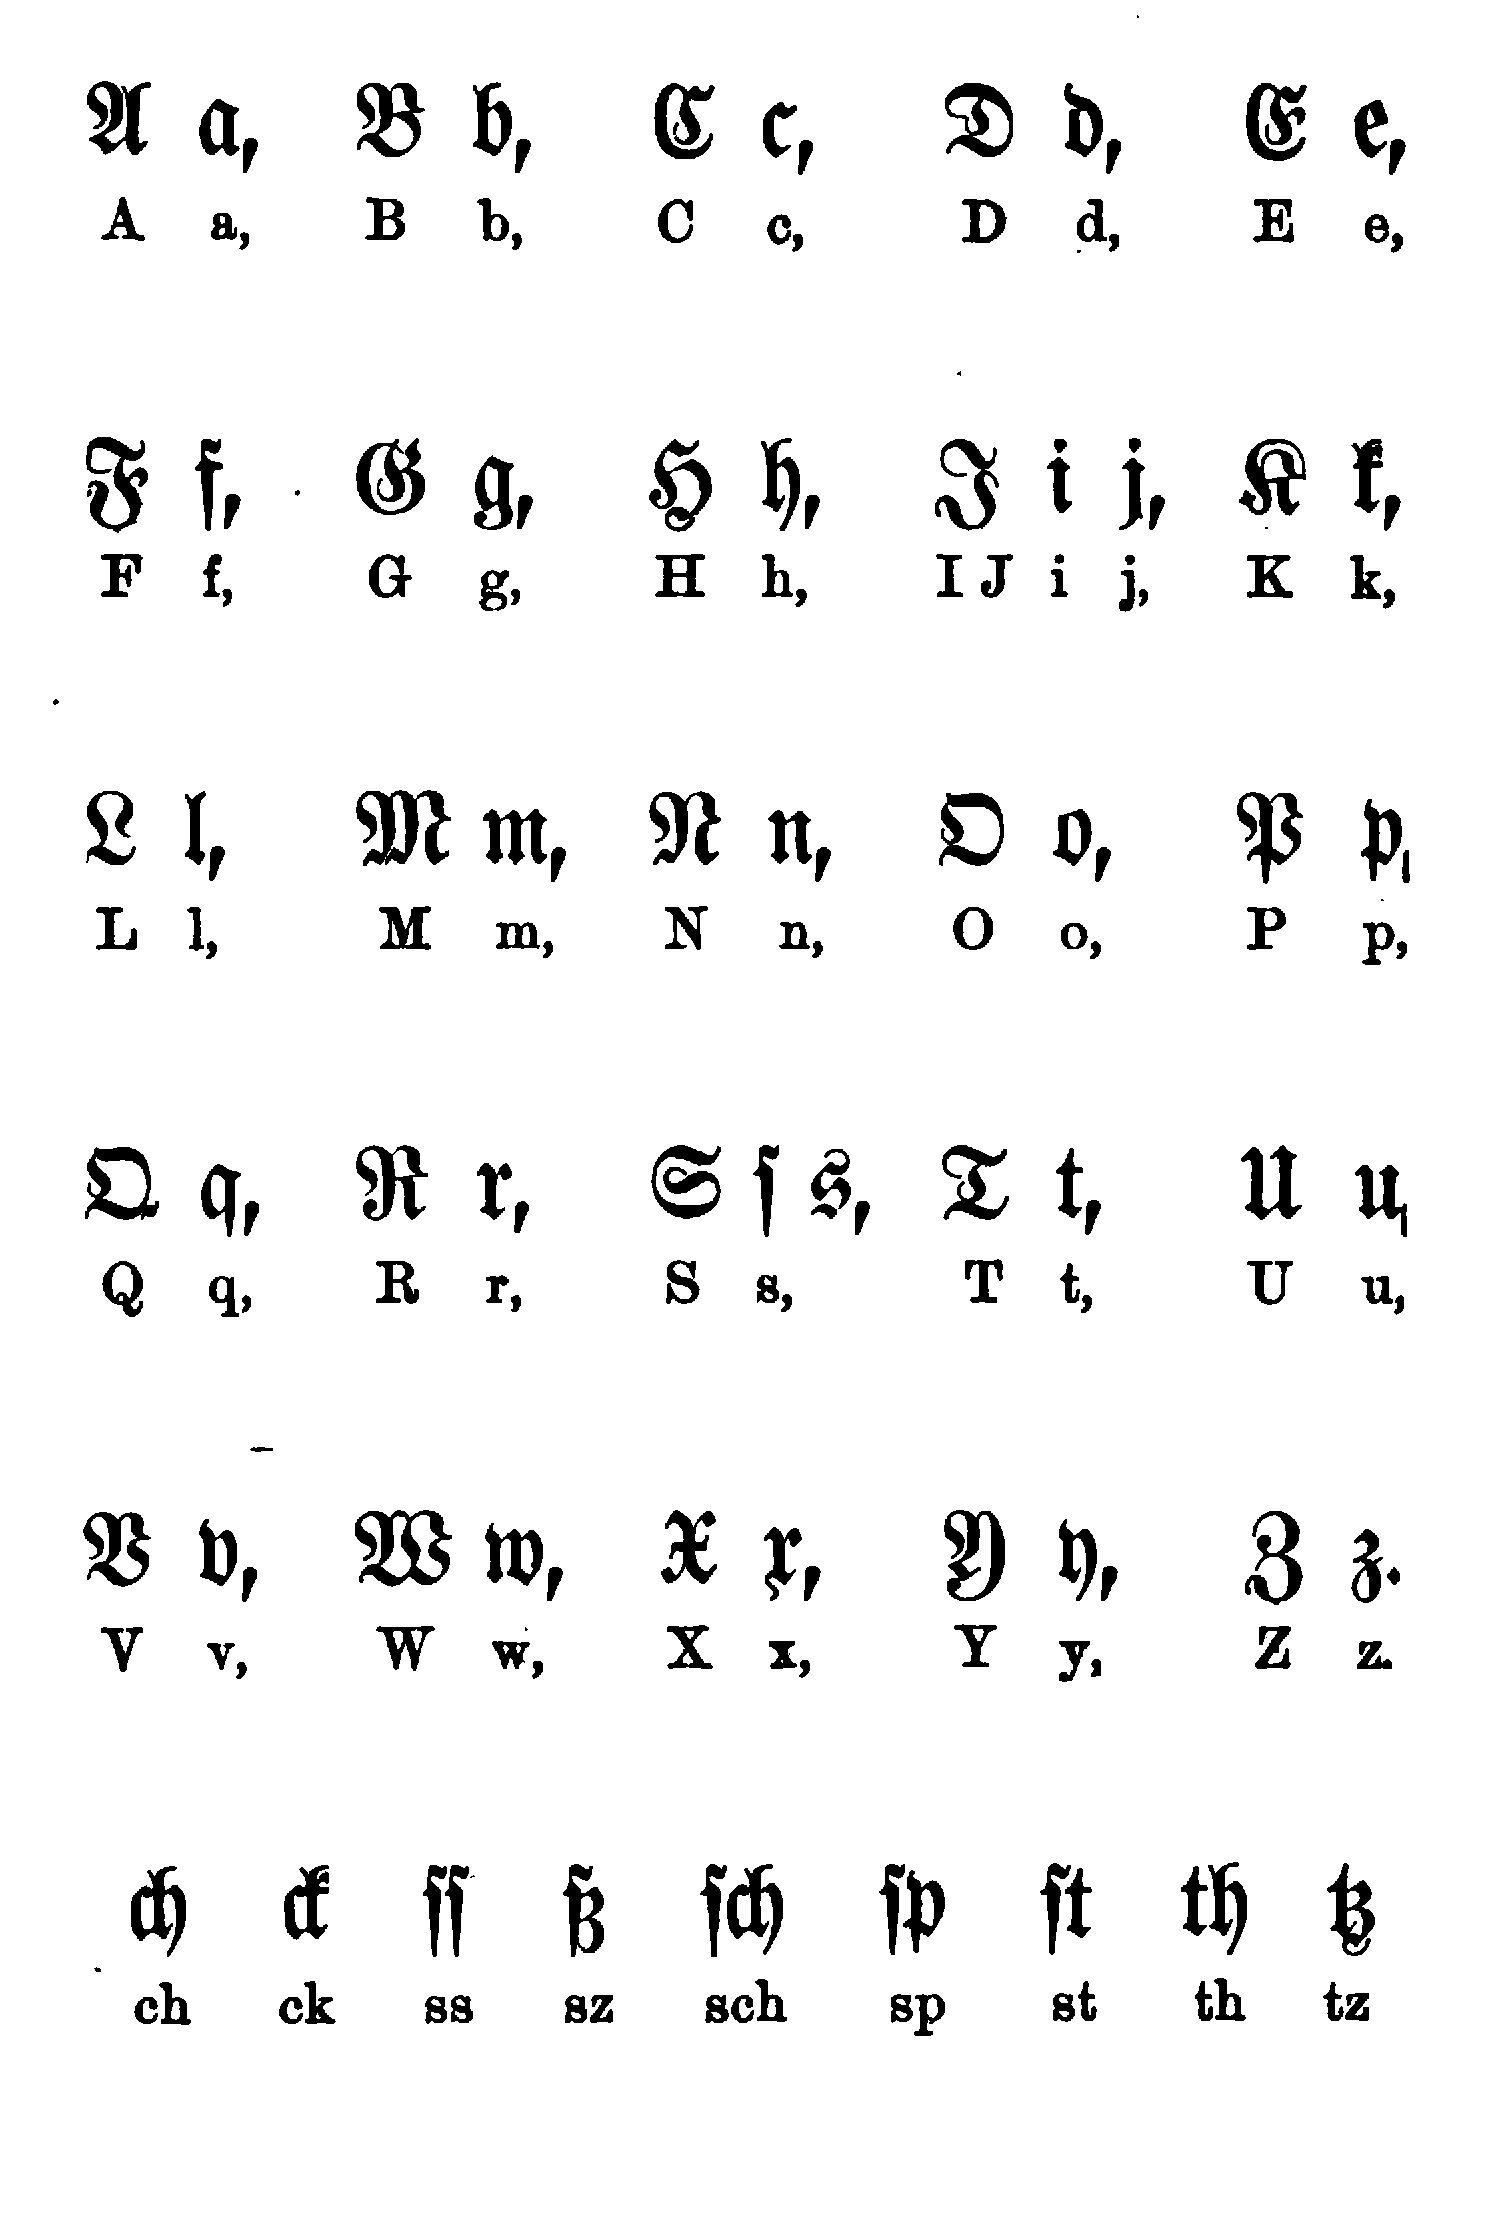
\includegraphics{german-Fraktur}
    \end{figure}

    \section*{Adjective Declensions}

    \begin{tcolorbox}[inflection,tabularx={Y|Y|Y|Y|Y},title={Strong Declensions},boxrule=0.5pt]
        Case       & Masculine Singular & Feminine Singular & Neuter Singular & All Genders Plural \\\hline\hline
        Nominative & {\German -er}      & {\German -e}      & {\German -es}   & {\German -e}       \\\hline
        Genitive   & {\German -en}      & {\German -er}     & {\German -en}   & {\German -er}      \\\hline
        Dative     & {\German -em}      & {\German -er}     & {\German -em}   & {\German -en}      \\\hline
        Accusative & {\German -en}      & {\German -e}      & {\German -es}   & {\German -e}       \\
    \end{tcolorbox}

    \begin{tcolorbox}[inflection,tabularx={Y|Y|Y|Y|Y},title={Weak Declensions {\German der, die, das}},boxrule=0.5pt]
        Case       & Masculine Singular & Feminine Singular & Neuter Singular & All Genders Plural \\\hline\hline
        Nominative & {\German -e}       & {\German -e}      & {\German -e}    & {\German -en}      \\\hline
        Genitive   & {\German -en}      & {\German -en}     & {\German -en}   & {\German -en}      \\\hline
        Dative     & {\German -en}      & {\German -en}     & {\German -en}   & {\German -en}      \\\hline
        Accusative & {\German -en}      & {\German -e}      & {\German -e}    & {\German -en}      \\
    \end{tcolorbox}

    \begin{tcolorbox}[inflection,tabularx={Y|Y|Y|Y|Y},title={Mixed Declensions {\German ein, kein, irgendein}},boxrule=0.5pt]
        Case       & Masculine Singular & Feminine Singular & Neuter Singular  & All Genders Plural \\\hline\hline
        Nominative & {\German -er}      & {\German -e}      & {\German -es}    & {\German -en}      \\\hline
        Genitive   & {\German -en}      & {\German -en}     & {\German -en}    & {\German -en}      \\\hline
        Dative     & {\German -en}      & {\German -en}     & {\German -en}    & {\German -en}      \\\hline
        Accusative & {\German -en}      & {\German -e}      & {\German -es}    & {\German -en}      \\
    \end{tcolorbox}

    \section*{Verb Conjugation}

    \begin{tcolorbox}[inflection,tabularx={Y|Y|Y},title={Present tense endings of weak verbs ending in {\German -en}},boxrule=0.5pt]
        Pronoun             & Verb ending in {\German -en}      & Verb ending in {\German -ern \& -eln} \\\hline\hline
        {\German ich}       & \multicolumn{2}{|c|}{\German -e}                                          \\\hline
        {\German du}        & \multicolumn{2}{|c|}{\German -st}                                         \\\hline
        {\German er/sie/es} & \multicolumn{2}{|c|}{\German -t}                                          \\\hline
        {\German wir}       & {\German -en}                     & {\German -n}                          \\\hline
        {\German ihr}       & \multicolumn{2}{|c|}{\German -t}                                          \\\hline
        {\German sie/Sie}   & {\German -en}                     & {\German -n}                          \\
    \end{tcolorbox}

    % VOCABULARY-START
    \section*{{\German der Raum} \href{https://upload.wikimedia.org/wikipedia/commons/9/94/De-Raum2.ogg}{
\includegraphics[width=0.05\textwidth]{audio}}}

\subsection*{Noun}

\begin{itemize}
    \item the room
    \item the area
    \item (Physics) the space
\end{itemize}

\subsubsection*{Declension}

\begin{tcolorbox}[inflection,tabularx={Y|Y|Y},title={Declension of {\German der Raum}},boxrule=0.5pt]
 & singular & plural \\\hline\hline
nominative & {\German Raum} & {\German Räume} \\\hline
genitive & {\German Raumes, Raums} & {\German Räume} \\\hline
dative & {\German Raum} & {\German Räumen} \\\hline
accusative & {\German Raum} & {\German Räume} \\
\end{tcolorbox}

    \section*{{\German der Begriff} \href{https://upload.wikimedia.org/wikipedia/commons/c/c2/De-Begriff.ogg}{
\includegraphics[width=0.05\textwidth]{audio}}}

\subsection*{Noun}

\begin{itemize}
    \item the term
    \item the word
    \item the idea
    \item the conception
    \item the perception
\end{itemize}

\subsubsection*{Declension}

\begin{tcolorbox}[inflection,tabularx={Y|Y|Y},title={Declension of {\German der Begriff}},boxrule=0.5pt]
 & singular & plural \\\hline\hline
Nominative & {\German Begriff} & {\German Begriffe} \\\hline
Genitive & {\German Begriffes, Begriffs} & {\German Begriffe} \\\hline
Dative & {\German Begriff} & {\German Begriffen} \\\hline
Accusative & {\German Begriff} & {\German Begriffe} \\
\end{tcolorbox}

    \section*{{\German der Abschnitt} \href{https://upload.wikimedia.org/wikipedia/commons/c/cf/De-Abschnitt.ogg}{
\includegraphics[width=0.05\textwidth]{audio}}}

\subsection*{Noun}

\begin{itemize}
    \item the section
    \item the paragraph
    \item the segment
\end{itemize}

\subsubsection*{Declension}

\begin{tcolorbox}[inflection,tabularx={Y|Y|Y},title={Declension of {\German der Abschnitt}},boxrule=0.5pt]
 & singular & plural \\\hline\hline
Nominative & {\German Abschnitt} & {\German Abschnitte} \\\hline
Genitive & {\German Abschnittes, Abschnitts} & {\German Abschnitte} \\\hline
Dative & {\German Abschnitt} & {\German Abschnitten} \\\hline
Accusative & {\German Abschnitt} & {\German Abschnitte} \\
\end{tcolorbox}

    \input{german/die Erörterung}
    \section*{{\German die Gleichzeitigkeit} \href{https://upload.wikimedia.org/wikipedia/commons/7/7a/De-Gleichzeitigkeit.ogg}{
\includegraphics[width=0.05\textwidth]{audio}}}

\subsection*{Noun}

\begin{itemize}
    \item the simultaneity
\end{itemize}

\subsubsection*{Declension}

\begin{tcolorbox}[inflection,tabularx={Y|Y|Y},title={Declension of {\German die Gleichzeitigkeit}},boxrule=0.5pt]
 & singular & plural \\\hline\hline
Nominative & {\German Gleichzeitigkeit} & N/A \\\hline
Genitive & {\German Gleichzeitigkeit} & N/A \\\hline
Dative & {\German Gleichzeitigkeit} & N/A \\\hline
Accusative & {\German Gleichzeitigkeit} & N/A \\
\end{tcolorbox}

    \section*{{\German das Koordinatensystem} \href{https://upload.wikimedia.org/wikipedia/commons/2/2d/De-Koordinatensystem.ogg}{
\includegraphics[width=0.05\textwidth]{audio}}}

\subsection*{Noun}

\begin{itemize}
    \item the coordinate system
\end{itemize}

\subsubsection*{Declension}

\begin{tcolorbox}[inflection,tabularx={Y|Y|Y},title={Declension of {\German das Koordinatensystem}},boxrule=0.5pt]
 & singular & plural \\\hline\hline
Nominative & {\German Koordinatensystem} & {\German Koordinatensysteme} \\\hline
Genitive & {\German Koordinatensystems} & {\German Koordinatensysteme} \\\hline
Dative & {\German Koordinatensystem} & {\German Koordinatensystemen} \\\hline
Accusative & {\German Koordinatensystem} & {\German Koordinatensysteme} \\
\end{tcolorbox}

    \section*{{\German die Gleichung} \href{https://upload.wikimedia.org/wikipedia/commons/9/95/De-Gleichung.ogg}{
\includegraphics[width=0.05\textwidth]{audio}}}

\subsection*{Noun}

\begin{itemize}
    \item the equation
    \item the equality
\end{itemize}

\subsubsection*{Declension}

\begin{tcolorbox}[inflection,tabularx={Y|Y|Y},title={Declension of {\German die Gleichung}},boxrule=0.5pt]
 & singular & plural \\\hline\hline
Nominative & {\German Gleichung} & {\German Gleichungen} \\\hline
Genitive & {\German Gleichung} & {\German Gleichungen} \\\hline
Dative & {\German Gleichung} & {\German Gleichungen} \\\hline
Accusative & {\German Gleichung} & {\German Gleichungen} \\
\end{tcolorbox}

    \section*{{\German die Erforschung} \href{https://upload.wikimedia.org/wikipedia/commons/4/45/De-Erforschung.ogg}{
\includegraphics[width=0.05\textwidth]{audio}}}

\subsection*{Noun}

\begin{itemize}
    \item the exploration
\end{itemize}

\subsubsection*{Declension}

\begin{tcolorbox}[inflection,tabularx={Y|Y|Y},title={Declension of {\German die Erforschung}},boxrule=0.5pt]
 & singular & plural \\\hline\hline
Nominative & {\German Erforschung} & {\German Erforschungen} \\\hline
Genitive & {\German Erforschung} & {\German Erforschungen} \\\hline
Dative & {\German Erforschung} & {\German Erforschungen} \\\hline
Accusative & {\German Erforschung} & {\German Erforschungen} \\
\end{tcolorbox}

    \section*{{\German die Behandlung} \href{https://upload.wikimedia.org/wikipedia/commons/f/ff/De-Behandlung.ogg}{
\includegraphics[width=0.05\textwidth]{audio}}}

\subsection*{Noun}

\begin{itemize}
    \item the treatment
\end{itemize}

\subsubsection*{Declension}

\begin{tcolorbox}[inflection,tabularx={Y|Y|Y},title={Declension of {\German die Behandlung}},boxrule=0.5pt]
 & singular & plural \\\hline\hline
nominative & {\German Behandlung} & {\German Behandlungen} \\\hline
genitive & {\German Behandlung} & {\German Behandlungen} \\\hline
dative & {\German Behandlung} & {\German Behandlungen} \\\hline
accusative & {\German Behandlung} & {\German Behandlungen} \\
\end{tcolorbox}

    \input{german/vorläufig}
    % VOCABULARY-END
\end{document}
